% Previous horizontal figure preserved for review:
% % Native TikZ source for the read-throughput heatmap.
% % Provenance: every cell is copied from throughput_ops_sec in
% %   vcomp/experiments/results/paper_figure4_uniform_read_cache_5m_single.tsv
% % (one 300-second run per cell).  The displayed K suffixes follow the former
% % PDF panel's compact human-readable formatting; exact promoted values are:
% %   Cached, ~0:     59153, 39, 156517, 120833, 68606, 76548
% %   Pinned, ~0:    669385, 3755, 713364, 452421, 420139, 694457
% %   Cached, 50GiB: 752969, 1579, 910711, 569202, 538646, 832889
% %   Pinned, 50GiB: 813716, 3883, 949618, 589071, 571893, 906821
% % Columns are Baseline, Flush-only, Last-comp, Fillseq, Fillseq+OW, F2Load.
% % Cell and legend colors are sampled from Matplotlib YlGnBu with LogNorm
% % vmin=30 and vmax=1,100,000, matching the superseded PDF panel.
% \definecolor{hmAOne}{HTML}{216AAD}
% \definecolor{hmATwo}{HTML}{FCFED1}
% \definecolor{hmAThree}{HTML}{24489D}
% \definecolor{hmAFour}{HTML}{2350A1}
% \definecolor{hmAFive}{HTML}{2163AA}
% \definecolor{hmASix}{HTML}{225EA8}
% \definecolor{hmCOne}{HTML}{13266F}
% \definecolor{hmCTwo}{HTML}{55BEC1}
% \definecolor{hmCThree}{HTML}{11246B}
% \definecolor{hmCFour}{HTML}{1B2C80}
% \definecolor{hmCFive}{HTML}{1D2E83}
% \definecolor{hmCSix}{HTML}{12256D}
% \definecolor{hmBOne}{HTML}{102369}
% \definecolor{hmBTwo}{HTML}{7ECDBB}
% \definecolor{hmBThree}{HTML}{0C2060}
% \definecolor{hmBFour}{HTML}{172976}
% \definecolor{hmBFive}{HTML}{172978}
% \definecolor{hmBSix}{HTML}{0D2163}
% \definecolor{hmDOne}{HTML}{0E2265}
% \definecolor{hmDTwo}{HTML}{53BDC1}
% \definecolor{hmDThree}{HTML}{0B1F5E}
% \definecolor{hmDFour}{HTML}{162874}
% \definecolor{hmDSix}{HTML}{0C2060}
% \definecolor{hmLegendOne}{HTML}{EFF9B5}
% \definecolor{hmLegendTwo}{HTML}{97D6B9}
% \definecolor{hmLegendThree}{HTML}{32A6C2}
% \definecolor{hmLegendFour}{HTML}{2356A4}
% \definecolor{hmLegendFive}{HTML}{0A1E5C}
% 
% \begin{tikzpicture}[
%     x=0.92cm,
%     y=0.66cm,
%     font=\sffamily\scriptsize,
%     heatcell/.style={draw=none, minimum width=0.92cm,
%                      minimum height=0.66cm, inner sep=0pt, outer sep=0pt}
% ]
% \path[use as bounding box] (-1.90,-1.22) rectangle (6.05,5.45);
% 
% % Five evenly spaced swatches represent equal decades on the logarithmic
% % color scale.  Their colors are sampled at the labeled throughputs.
% \node[font=\sffamily\scriptsize] at (3.00,5.25)
%     {Throughput (ops/s; log color)};
% \foreach \xa/\xb/\fillcolor/\tick in {
%     0.50/1.50/hmLegendOne/100,
%     1.50/2.50/hmLegendTwo/1K,
%     2.50/3.50/hmLegendThree/10K,
%     3.50/4.50/hmLegendFour/100K,
%     4.50/5.50/hmLegendFive/1M
% } {
%     \draw[draw=black!45, line width=0.3pt, fill=\fillcolor]
%         (\xa,4.69) rectangle (\xb,4.96);
%     \node[font=\sffamily\tiny, anchor=north] at ({(\xa+\xb)/2},4.65) {\tick};
% }
% 
% % Cached metadata, effectively zero data cache (the experiment uses 1 byte).
% \node[align=right, anchor=east] at (-0.10,3.50) {Cached, $\approx$0};
% \node[heatcell, fill=hmAOne, text=white]   at (0.50,3.50) {59.2K};
% \node[heatcell, fill=hmATwo, text=black]   at (1.50,3.50) {39};
% \node[heatcell, fill=hmAThree, text=white] at (2.50,3.50) {157K};
% \node[heatcell, fill=hmAFour, text=white]  at (3.50,3.50) {121K};
% \node[heatcell, fill=hmAFive, text=white]  at (4.50,3.50) {68.6K};
% \node[heatcell, fill=hmASix, text=white]   at (5.50,3.50) {76.5K};
% 
% % Pinned filter/index metadata, effectively zero data cache (1 byte).
% \node[align=right, anchor=east] at (-0.10,2.50) {Pinned, $\approx$0};
% \node[heatcell, fill=hmCOne, text=white]   at (0.50,2.50) {669K};
% \node[heatcell, fill=hmCTwo, text=black]   at (1.50,2.50) {3.8K};
% \node[heatcell, fill=hmCThree, text=white] at (2.50,2.50) {713K};
% \node[heatcell, fill=hmCFour, text=white]  at (3.50,2.50) {452K};
% \node[heatcell, fill=hmCFive, text=white]  at (4.50,2.50) {420K};
% \node[heatcell, fill=hmCSix, text=white]   at (5.50,2.50) {694K};
% 
% % Cached filter/index metadata and a 50 GiB block cache.
% \node[align=right, anchor=east] at (-0.10,1.50) {Cached, 50~GiB};
% \node[heatcell, fill=hmBOne, text=white]   at (0.50,1.50) {753K};
% \node[heatcell, fill=hmBTwo, text=black]   at (1.50,1.50) {1.6K};
% \node[heatcell, fill=hmBThree, text=white] at (2.50,1.50) {911K};
% \node[heatcell, fill=hmBFour, text=white]  at (3.50,1.50) {569K};
% \node[heatcell, fill=hmBFive, text=white]  at (4.50,1.50) {539K};
% \node[heatcell, fill=hmBSix, text=white]   at (5.50,1.50) {833K};
% 
% % Pinned filter/index metadata and a 50 GiB data-block cache.
% \node[align=right, anchor=east] at (-0.10,0.50) {Pinned, 50~GiB};
% \node[heatcell, fill=hmDOne, text=white]   at (0.50,0.50) {814K};
% \node[heatcell, fill=hmDTwo, text=black]   at (1.50,0.50) {3.9K};
% \node[heatcell, fill=hmDThree, text=white] at (2.50,0.50) {950K};
% \node[heatcell, fill=hmDFour, text=white]  at (3.50,0.50) {589K};
% \node[heatcell, fill=hmDFour, text=white]  at (4.50,0.50) {572K};
% \node[heatcell, fill=hmDSix, text=white]   at (5.50,0.50) {907K};
% 
% % Cell boundaries are explicit so adjacent equal-colored cells remain visible.
% \foreach \row in {0,...,3} {
%     \foreach \col in {0,...,5} {
%         \draw[black!55, line width=0.35pt]
%             (\col,\row) rectangle ({\col+1},{\row+1});
%     }
% }
% 
% \foreach \x/\label in {
%     0.50/Base,
%     1.50/Flush,
%     2.50/Last,
%     3.50/Seq,
%     4.50/{Seq+OW},
%     5.50/F2Load
% } {
%     \node[font=\sffamily\scriptsize, rotate=35, anchor=north east]
%         at (\x,-0.10) {\label};
% }
% \end{tikzpicture}

% Previous plotted version preserved for review:
% % Loading: vcomp/experiments/results/paper_figure4_loading_time_1tb_single.tsv
% % Reads: vcomp/experiments/results/paper_figure4_uniform_read_cache_5m_single.tsv
% % One run per cell; all measured values are unchanged by this layout revision.
% \begingroup
% \definecolor{vb0}{HTML}{4477AA}
% \definecolor{vb1}{HTML}{66CCEE}
% \definecolor{vb2}{HTML}{EE6677}
% \definecolor{vb3}{HTML}{CCBB44}
% \begin{tikzpicture}[x=1cm,y=1cm,font=\small,
% axis/.style={draw=black!80,line width=0.5pt},
% grid/.style={draw=black!16,line width=0.4pt}]
% \path[use as bounding box] (0,0) rectangle (7.200,5.650);
% \draw[grid] (0.85,1.4000) -- (7.1000,1.4000);
% \draw[axis] (0.79,1.4000) -- (0.85,1.4000);
% \node[font=\fontsize{7}{8}\selectfont,anchor=east] at (0.7300,1.4000) {10};
% \draw[grid] (0.85,2.0453) -- (7.1000,2.0453);
% \draw[axis] (0.79,2.0453) -- (0.85,2.0453);
% \node[font=\fontsize{7}{8}\selectfont,anchor=east] at (0.7300,2.0453) {100};
% \draw[grid] (0.85,2.6906) -- (7.1000,2.6906);
% \draw[axis] (0.79,2.6906) -- (0.85,2.6906);
% \node[font=\fontsize{7}{8}\selectfont,anchor=east] at (0.7300,2.6906) {1K};
% \draw[grid] (0.85,3.3359) -- (7.1000,3.3359);
% \draw[axis] (0.79,3.3359) -- (0.85,3.3359);
% \node[font=\fontsize{7}{8}\selectfont,anchor=east] at (0.7300,3.3359) {10K};
% \draw[grid] (0.85,3.9812) -- (7.1000,3.9812);
% \draw[axis] (0.79,3.9812) -- (0.85,3.9812);
% \node[font=\fontsize{7}{8}\selectfont,anchor=east] at (0.7300,3.9812) {100K};
% \draw[grid] (0.85,4.6265) -- (7.1000,4.6265);
% \draw[axis] (0.79,4.6265) -- (0.85,4.6265);
% \node[font=\fontsize{7}{8}\selectfont,anchor=east] at (0.7300,4.6265) {1M};
% \draw[axis] (0.85,1.4000) -- (7.1000,1.4000);
% \draw[axis] (0.85,1.4000) -- (0.85,4.7000);
% \node[font=\fontsize{7}{8}\selectfont,rotate=90,anchor=south] at (0.1000,3.0500) {Throughput (ops/s; log)};
% % baseline / A_cache_zero: 59153.000000 ops/s
% \draw[draw=black!80,line width=0.4pt,fill=vb0] (1.03000,1.40000) rectangle (1.20000,3.83404);
% % baseline / C_pinned_zero: 669385.000000 ops/s
% \draw[draw=black!80,line width=0.4pt,fill=vb1] (1.22000,1.40000) rectangle (1.39000,4.51398);
% % baseline / B_cache_5pct: 752969.000000 ops/s
% \draw[draw=black!80,line width=0.4pt,fill=vb2] (1.41000,1.40000) rectangle (1.58000,4.54696);
% % baseline / D_pinned_5pct: 813716.000000 ops/s
% \draw[draw=black!80,line width=0.4pt,fill=vb3] (1.60000,1.40000) rectangle (1.77000,4.56870);
% \node[font=\fontsize{7}{8}\selectfont,rotate=55,anchor=north east] at (1.4000,1.3000) {Baseline};
% % flush_only / A_cache_zero: 39.000000 ops/s
% \draw[draw=black!80,line width=0.4pt,fill=vb0] (2.07000,1.40000) rectangle (2.24000,1.78141);
% % flush_only / C_pinned_zero: 3755.000000 ops/s
% \draw[draw=black!80,line width=0.4pt,fill=vb1] (2.26000,1.40000) rectangle (2.43000,3.06138);
% % flush_only / B_cache_5pct: 1579.000000 ops/s
% \draw[draw=black!80,line width=0.4pt,fill=vb2] (2.45000,1.40000) rectangle (2.62000,2.81860);
% % flush_only / D_pinned_5pct: 3883.000000 ops/s
% \draw[draw=black!80,line width=0.4pt,fill=vb3] (2.64000,1.40000) rectangle (2.81000,3.07078);
% \node[font=\fontsize{7}{8}\selectfont,rotate=55,anchor=north east] at (2.4400,1.3000) {Flush-only};
% % last_comp / A_cache_zero: 156517.000000 ops/s
% \draw[draw=black!80,line width=0.4pt,fill=vb0] (3.11000,1.40000) rectangle (3.28000,4.10673);
% % last_comp / C_pinned_zero: 713364.000000 ops/s
% \draw[draw=black!80,line width=0.4pt,fill=vb1] (3.30000,1.40000) rectangle (3.47000,4.53182);
% % last_comp / B_cache_5pct: 910711.000000 ops/s
% \draw[draw=black!80,line width=0.4pt,fill=vb2] (3.49000,1.40000) rectangle (3.66000,4.60026);
% % last_comp / D_pinned_5pct: 949618.000000 ops/s
% \draw[draw=black!80,line width=0.4pt,fill=vb3] (3.68000,1.40000) rectangle (3.85000,4.61199);
% \node[font=\fontsize{7}{8}\selectfont,rotate=55,anchor=north east] at (3.4800,1.3000) {Last-comp};
% % fillseq / A_cache_zero: 120833.000000 ops/s
% \draw[draw=black!80,line width=0.4pt,fill=vb0] (4.15000,1.40000) rectangle (4.32000,4.03421);
% % fillseq / C_pinned_zero: 452421.000000 ops/s
% \draw[draw=black!80,line width=0.4pt,fill=vb1] (4.34000,1.40000) rectangle (4.51000,4.40420);
% % fillseq / B_cache_5pct: 569202.000000 ops/s
% \draw[draw=black!80,line width=0.4pt,fill=vb2] (4.53000,1.40000) rectangle (4.70000,4.46855);
% % fillseq / D_pinned_5pct: 589071.000000 ops/s
% \draw[draw=black!80,line width=0.4pt,fill=vb3] (4.72000,1.40000) rectangle (4.89000,4.47816);
% \node[font=\fontsize{7}{8}\selectfont,rotate=55,anchor=north east] at (4.5200,1.3000) {Fillseq};
% % fillseq_ow / A_cache_zero: 68606.000000 ops/s
% \draw[draw=black!80,line width=0.4pt,fill=vb0] (5.19000,1.40000) rectangle (5.36000,3.87558);
% % fillseq_ow / C_pinned_zero: 420139.000000 ops/s
% \draw[draw=black!80,line width=0.4pt,fill=vb1] (5.38000,1.40000) rectangle (5.55000,4.38345);
% % fillseq_ow / B_cache_5pct: 538646.000000 ops/s
% \draw[draw=black!80,line width=0.4pt,fill=vb2] (5.57000,1.40000) rectangle (5.74000,4.45308);
% % fillseq_ow / D_pinned_5pct: 571893.000000 ops/s
% \draw[draw=black!80,line width=0.4pt,fill=vb3] (5.76000,1.40000) rectangle (5.93000,4.46987);
% \node[font=\fontsize{7}{8}\selectfont,rotate=55,anchor=north east] at (5.5600,1.3000) {Fillseq+OW};
% % f2load / A_cache_zero: 76548.000000 ops/s
% \draw[draw=black!80,line width=0.4pt,fill=vb0] (6.23000,1.40000) rectangle (6.40000,3.90628);
% % f2load / C_pinned_zero: 694457.000000 ops/s
% \draw[draw=black!80,line width=0.4pt,fill=vb1] (6.42000,1.40000) rectangle (6.59000,4.52429);
% % f2load / B_cache_5pct: 832889.000000 ops/s
% \draw[draw=black!80,line width=0.4pt,fill=vb2] (6.61000,1.40000) rectangle (6.78000,4.57523);
% % f2load / D_pinned_5pct: 906821.000000 ops/s
% \draw[draw=black!80,line width=0.4pt,fill=vb3] (6.80000,1.40000) rectangle (6.97000,4.59906);
% \node[font=\fontsize{7}{8}\selectfont,rotate=55,anchor=north east] at (6.6000,1.3000) {F2Load};
% \draw[draw=black!80,line width=0.4pt,fill=vb0] (1.40000,5.30000) rectangle (1.63000,5.46000);
% \node[font=\fontsize{7}{8}\selectfont,anchor=west] at (1.7400,5.3800) {Cached, $\approx$0};
% \draw[draw=black!80,line width=0.4pt,fill=vb1] (4.15000,5.30000) rectangle (4.38000,5.46000);
% \node[font=\fontsize{7}{8}\selectfont,anchor=west] at (4.4900,5.3800) {Pinned, $\approx$0};
% \draw[draw=black!80,line width=0.4pt,fill=vb2] (1.40000,5.00000) rectangle (1.63000,5.16000);
% \node[font=\fontsize{7}{8}\selectfont,anchor=west] at (1.7400,5.0800) {Cached, 50 GiB};
% \draw[draw=black!80,line width=0.4pt,fill=vb3] (4.15000,5.00000) rectangle (4.38000,5.16000);
% \node[font=\fontsize{7}{8}\selectfont,anchor=west] at (4.4900,5.0800) {Pinned, 50 GiB};
% \end{tikzpicture}
% \endgroup

% Previous plotted version preserved for review:
% % Loading: vcomp/experiments/results/paper_figure4_loading_time_1tb_single.tsv
% % Reads: vcomp/experiments/results/paper_figure4_uniform_read_cache_5m_single.tsv
% % One run per cell; all measured values are unchanged by this layout revision.
% \begingroup
% \definecolor{vb0}{HTML}{4477AA}
% \definecolor{vb1}{HTML}{66CCEE}
% \definecolor{vb2}{HTML}{EE6677}
% \definecolor{vb3}{HTML}{CCBB44}
% \begin{tikzpicture}[x=1cm,y=1cm,font=\small,
% axis/.style={draw=black!80,line width=0.5pt},
% grid/.style={draw=black!16,line width=0.4pt}]
% \path[use as bounding box] (0,0) rectangle (7.200,5.650);
% \draw[grid] (0.85,1.4000) -- (7.1000,1.4000);
% \draw[axis] (0.79,1.4000) -- (0.85,1.4000);
% \node[font=\fontsize{7}{8}\selectfont,anchor=east] at (0.7300,1.4000) {0};
% \draw[grid] (0.85,2.5000) -- (7.1000,2.5000);
% \draw[axis] (0.79,2.5000) -- (0.85,2.5000);
% \node[font=\fontsize{7}{8}\selectfont,anchor=east] at (0.7300,2.5000) {1};
% \draw[grid] (0.85,3.6000) -- (7.1000,3.6000);
% \draw[axis] (0.79,3.6000) -- (0.85,3.6000);
% \node[font=\fontsize{7}{8}\selectfont,anchor=east] at (0.7300,3.6000) {2};
% \draw[grid] (0.85,4.7000) -- (7.1000,4.7000);
% \draw[axis] (0.79,4.7000) -- (0.85,4.7000);
% \node[font=\fontsize{7}{8}\selectfont,anchor=east] at (0.7300,4.7000) {3};
% \draw[axis] (0.85,1.4000) -- (7.1000,1.4000);
% \draw[axis] (0.85,1.4000) -- (0.85,4.7000);
% \node[font=\fontsize{7}{8}\selectfont,rotate=90,anchor=south] at (0.1000,3.0500) {Throughput / Baseline};
% % baseline / A_cache_zero: 59153.000000 ops/s, baseline=59153.000000 ops/s, normalized=1.000000000
% \draw[draw=black!80,line width=0.4pt,fill=vb0] (1.03000,1.40000) rectangle (1.20000,2.50000);
% % baseline / C_pinned_zero: 669385.000000 ops/s, baseline=669385.000000 ops/s, normalized=1.000000000
% \draw[draw=black!80,line width=0.4pt,fill=vb1] (1.22000,1.40000) rectangle (1.39000,2.50000);
% % baseline / B_cache_5pct: 752969.000000 ops/s, baseline=752969.000000 ops/s, normalized=1.000000000
% \draw[draw=black!80,line width=0.4pt,fill=vb2] (1.41000,1.40000) rectangle (1.58000,2.50000);
% % baseline / D_pinned_5pct: 813716.000000 ops/s, baseline=813716.000000 ops/s, normalized=1.000000000
% \draw[draw=black!80,line width=0.4pt,fill=vb3] (1.60000,1.40000) rectangle (1.77000,2.50000);
% \node[font=\fontsize{7}{8}\selectfont,rotate=55,anchor=north east] at (1.4000,1.3000) {Baseline};
% % flush_only / A_cache_zero: 39.000000 ops/s, baseline=59153.000000 ops/s, normalized=0.000659307
% \draw[draw=black!80,line width=0.4pt,fill=vb0] (2.07000,1.40000) rectangle (2.24000,1.40073);
% % flush_only / C_pinned_zero: 3755.000000 ops/s, baseline=669385.000000 ops/s, normalized=0.005609627
% \draw[draw=black!80,line width=0.4pt,fill=vb1] (2.26000,1.40000) rectangle (2.43000,1.40617);
% % flush_only / B_cache_5pct: 1579.000000 ops/s, baseline=752969.000000 ops/s, normalized=0.002097032
% \draw[draw=black!80,line width=0.4pt,fill=vb2] (2.45000,1.40000) rectangle (2.62000,1.40231);
% % flush_only / D_pinned_5pct: 3883.000000 ops/s, baseline=813716.000000 ops/s, normalized=0.004771935
% \draw[draw=black!80,line width=0.4pt,fill=vb3] (2.64000,1.40000) rectangle (2.81000,1.40525);
% \node[font=\fontsize{7}{8}\selectfont,anchor=south] at (2.4400,1.5430) {$<0.006$};
% \node[font=\fontsize{7}{8}\selectfont,rotate=55,anchor=north east] at (2.4400,1.3000) {Flush-only};
% % last_comp / A_cache_zero: 156517.000000 ops/s, baseline=59153.000000 ops/s, normalized=2.645968928
% \draw[draw=black!80,line width=0.4pt,fill=vb0] (3.11000,1.40000) rectangle (3.28000,4.31057);
% % last_comp / C_pinned_zero: 713364.000000 ops/s, baseline=669385.000000 ops/s, normalized=1.065700606
% \draw[draw=black!80,line width=0.4pt,fill=vb1] (3.30000,1.40000) rectangle (3.47000,2.57227);
% % last_comp / B_cache_5pct: 910711.000000 ops/s, baseline=752969.000000 ops/s, normalized=1.209493352
% \draw[draw=black!80,line width=0.4pt,fill=vb2] (3.49000,1.40000) rectangle (3.66000,2.73044);
% % last_comp / D_pinned_5pct: 949618.000000 ops/s, baseline=813716.000000 ops/s, normalized=1.167014044
% \draw[draw=black!80,line width=0.4pt,fill=vb3] (3.68000,1.40000) rectangle (3.85000,2.68372);
% \node[font=\fontsize{7}{8}\selectfont,rotate=55,anchor=north east] at (3.4800,1.3000) {Last-comp};
% % fillseq / A_cache_zero: 120833.000000 ops/s, baseline=59153.000000 ops/s, normalized=2.042719727
% \draw[draw=black!80,line width=0.4pt,fill=vb0] (4.15000,1.40000) rectangle (4.32000,3.64699);
% % fillseq / C_pinned_zero: 452421.000000 ops/s, baseline=669385.000000 ops/s, normalized=0.675875617
% \draw[draw=black!80,line width=0.4pt,fill=vb1] (4.34000,1.40000) rectangle (4.51000,2.14346);
% % fillseq / B_cache_5pct: 569202.000000 ops/s, baseline=752969.000000 ops/s, normalized=0.755943472
% \draw[draw=black!80,line width=0.4pt,fill=vb2] (4.53000,1.40000) rectangle (4.70000,2.23154);
% % fillseq / D_pinned_5pct: 589071.000000 ops/s, baseline=813716.000000 ops/s, normalized=0.723927021
% \draw[draw=black!80,line width=0.4pt,fill=vb3] (4.72000,1.40000) rectangle (4.89000,2.19632);
% \node[font=\fontsize{7}{8}\selectfont,rotate=55,anchor=north east] at (4.5200,1.3000) {Fillseq};
% % fillseq_ow / A_cache_zero: 68606.000000 ops/s, baseline=59153.000000 ops/s, normalized=1.159805927
% \draw[draw=black!80,line width=0.4pt,fill=vb0] (5.19000,1.40000) rectangle (5.36000,2.67579);
% % fillseq_ow / C_pinned_zero: 420139.000000 ops/s, baseline=669385.000000 ops/s, normalized=0.627649260
% \draw[draw=black!80,line width=0.4pt,fill=vb1] (5.38000,1.40000) rectangle (5.55000,2.09041);
% % fillseq_ow / B_cache_5pct: 538646.000000 ops/s, baseline=752969.000000 ops/s, normalized=0.715362784
% \draw[draw=black!80,line width=0.4pt,fill=vb2] (5.57000,1.40000) rectangle (5.74000,2.18690);
% % fillseq_ow / D_pinned_5pct: 571893.000000 ops/s, baseline=813716.000000 ops/s, normalized=0.702816462
% \draw[draw=black!80,line width=0.4pt,fill=vb3] (5.76000,1.40000) rectangle (5.93000,2.17310);
% \node[font=\fontsize{7}{8}\selectfont,rotate=55,anchor=north east] at (5.5600,1.3000) {Fillseq+OW};
% % f2load / A_cache_zero: 76548.000000 ops/s, baseline=59153.000000 ops/s, normalized=1.294067926
% \draw[draw=black!80,line width=0.4pt,fill=vb0] (6.23000,1.40000) rectangle (6.40000,2.82347);
% % f2load / C_pinned_zero: 694457.000000 ops/s, baseline=669385.000000 ops/s, normalized=1.037455276
% \draw[draw=black!80,line width=0.4pt,fill=vb1] (6.42000,1.40000) rectangle (6.59000,2.54120);
% % f2load / B_cache_5pct: 832889.000000 ops/s, baseline=752969.000000 ops/s, normalized=1.106139828
% \draw[draw=black!80,line width=0.4pt,fill=vb2] (6.61000,1.40000) rectangle (6.78000,2.61675);
% % f2load / D_pinned_5pct: 906821.000000 ops/s, baseline=813716.000000 ops/s, normalized=1.114419527
% \draw[draw=black!80,line width=0.4pt,fill=vb3] (6.80000,1.40000) rectangle (6.97000,2.62586);
% \node[font=\fontsize{7}{8}\selectfont,rotate=55,anchor=north east] at (6.6000,1.3000) {F2Load};
% \draw[red,line width=0.8pt] (0.85,2.5000) -- (7.10,2.5000);
% \draw[draw=black!80,line width=0.4pt,fill=vb0] (1.40000,5.30000) rectangle (1.63000,5.46000);
% \node[font=\fontsize{7}{8}\selectfont,anchor=west] at (1.7400,5.3800) {Cached, $\approx$0};
% \draw[draw=black!80,line width=0.4pt,fill=vb1] (4.15000,5.30000) rectangle (4.38000,5.46000);
% \node[font=\fontsize{7}{8}\selectfont,anchor=west] at (4.4900,5.3800) {Pinned, $\approx$0};
% \draw[draw=black!80,line width=0.4pt,fill=vb2] (1.40000,5.00000) rectangle (1.63000,5.16000);
% \node[font=\fontsize{7}{8}\selectfont,anchor=west] at (1.7400,5.0800) {Cached, 50 GiB};
% \draw[draw=black!80,line width=0.4pt,fill=vb3] (4.15000,5.00000) rectangle (4.38000,5.16000);
% \node[font=\fontsize{7}{8}\selectfont,anchor=west] at (4.4900,5.0800) {Pinned, 50 GiB};
% \end{tikzpicture}
% \endgroup

% Active vertical figure generated from the promoted TSV data.
% Loading: vcomp/experiments/results/paper_figure4_loading_time_1tb_single.tsv
% Reads: vcomp/experiments/results/paper_figure4_uniform_read_cache_5m_single.tsv
% One run per cell; labels, membership and ratios derive from the TSV inputs.
\begingroup
\definecolor{vb0}{HTML}{4477AA}
\definecolor{vb1}{HTML}{66CCEE}
\definecolor{vb2}{HTML}{EE6677}
\definecolor{vb3}{HTML}{CCBB44}
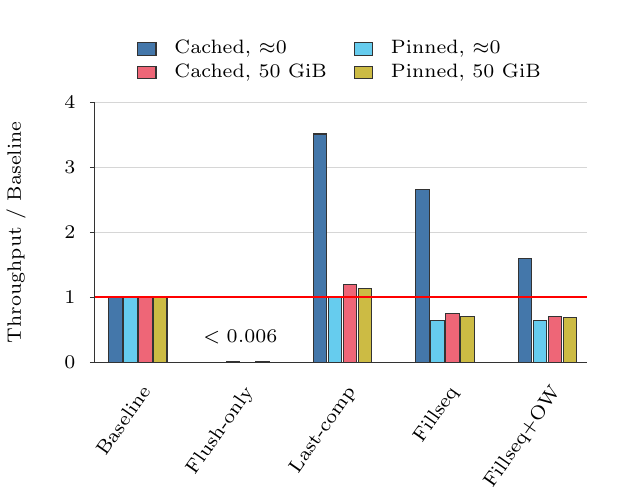
\begin{tikzpicture}[x=1cm,y=1cm,font=\small,
axis/.style={draw=black!80,line width=0.5pt},
grid/.style={draw=black!16,line width=0.4pt}]
\path[use as bounding box] (0,0) rectangle (7.200,5.650);
\draw[grid] (0.85,1.4000) -- (7.1000,1.4000);
\draw[axis] (0.79,1.4000) -- (0.85,1.4000);
\node[font=\fontsize{7}{8}\selectfont,anchor=east] at (0.7300,1.4000) {0};
\draw[grid] (0.85,2.2250) -- (7.1000,2.2250);
\draw[axis] (0.79,2.2250) -- (0.85,2.2250);
\node[font=\fontsize{7}{8}\selectfont,anchor=east] at (0.7300,2.2250) {1};
\draw[grid] (0.85,3.0500) -- (7.1000,3.0500);
\draw[axis] (0.79,3.0500) -- (0.85,3.0500);
\node[font=\fontsize{7}{8}\selectfont,anchor=east] at (0.7300,3.0500) {2};
\draw[grid] (0.85,3.8750) -- (7.1000,3.8750);
\draw[axis] (0.79,3.8750) -- (0.85,3.8750);
\node[font=\fontsize{7}{8}\selectfont,anchor=east] at (0.7300,3.8750) {3};
\draw[grid] (0.85,4.7000) -- (7.1000,4.7000);
\draw[axis] (0.79,4.7000) -- (0.85,4.7000);
\node[font=\fontsize{7}{8}\selectfont,anchor=east] at (0.7300,4.7000) {4};
\draw[axis] (0.85,1.4000) -- (7.1000,1.4000);
\draw[axis] (0.85,1.4000) -- (0.85,4.7000);
\node[font=\fontsize{7}{8}\selectfont,rotate=90,anchor=south] at (0.1000,3.0500) {Throughput / Baseline};
% baseline / A_cache_zero: 45751.000000 ops/s, baseline=45751.000000 ops/s, normalized=1.000000000
\draw[draw=black!80,line width=0.4pt,fill=vb0] (1.03000,1.40000) rectangle (1.20000,2.22500);
% baseline / C_pinned_zero: 685109.000000 ops/s, baseline=685109.000000 ops/s, normalized=1.000000000
\draw[draw=black!80,line width=0.4pt,fill=vb1] (1.22000,1.40000) rectangle (1.39000,2.22500);
% baseline / B_cache_5pct: 757310.000000 ops/s, baseline=757310.000000 ops/s, normalized=1.000000000
\draw[draw=black!80,line width=0.4pt,fill=vb2] (1.41000,1.40000) rectangle (1.58000,2.22500);
% baseline / D_pinned_5pct: 826749.000000 ops/s, baseline=826749.000000 ops/s, normalized=1.000000000
\draw[draw=black!80,line width=0.4pt,fill=vb3] (1.60000,1.40000) rectangle (1.77000,2.22500);
\node[font=\fontsize{7}{8}\selectfont,rotate=55,anchor=north east] at (1.4000,1.3000) {Baseline};
% flush_only / A_cache_zero: 39.000000 ops/s, baseline=45751.000000 ops/s, normalized=0.000852440
\draw[draw=black!80,line width=0.4pt,fill=vb0] (2.33000,1.40000) rectangle (2.50000,1.40070);
% flush_only / C_pinned_zero: 3642.000000 ops/s, baseline=685109.000000 ops/s, normalized=0.005315942
\draw[draw=black!80,line width=0.4pt,fill=vb1] (2.52000,1.40000) rectangle (2.69000,1.40439);
% flush_only / B_cache_5pct: 1550.000000 ops/s, baseline=757310.000000 ops/s, normalized=0.002046718
\draw[draw=black!80,line width=0.4pt,fill=vb2] (2.71000,1.40000) rectangle (2.88000,1.40169);
% flush_only / D_pinned_5pct: 3690.000000 ops/s, baseline=826749.000000 ops/s, normalized=0.004463265
\draw[draw=black!80,line width=0.4pt,fill=vb3] (2.90000,1.40000) rectangle (3.07000,1.40368);
\node[font=\fontsize{7}{8}\selectfont,anchor=south] at (2.7000,1.5072) {$<0.006$};
\node[font=\fontsize{7}{8}\selectfont,rotate=55,anchor=north east] at (2.7000,1.3000) {Flush-only};
% last_comp / A_cache_zero: 160800.000000 ops/s, baseline=45751.000000 ops/s, normalized=3.514677275
\draw[draw=black!80,line width=0.4pt,fill=vb0] (3.63000,1.40000) rectangle (3.80000,4.29961);
% last_comp / C_pinned_zero: 692628.000000 ops/s, baseline=685109.000000 ops/s, normalized=1.010974896
\draw[draw=black!80,line width=0.4pt,fill=vb1] (3.82000,1.40000) rectangle (3.99000,2.23405);
% last_comp / B_cache_5pct: 902532.000000 ops/s, baseline=757310.000000 ops/s, normalized=1.191760310
\draw[draw=black!80,line width=0.4pt,fill=vb2] (4.01000,1.40000) rectangle (4.18000,2.38320);
% last_comp / D_pinned_5pct: 940142.000000 ops/s, baseline=826749.000000 ops/s, normalized=1.137155291
\draw[draw=black!80,line width=0.4pt,fill=vb3] (4.20000,1.40000) rectangle (4.37000,2.33815);
\node[font=\fontsize{7}{8}\selectfont,rotate=55,anchor=north east] at (4.0000,1.3000) {Last-comp};
% fillseq / A_cache_zero: 121787.000000 ops/s, baseline=45751.000000 ops/s, normalized=2.661952744
\draw[draw=black!80,line width=0.4pt,fill=vb0] (4.93000,1.40000) rectangle (5.10000,3.59611);
% fillseq / C_pinned_zero: 438079.000000 ops/s, baseline=685109.000000 ops/s, normalized=0.639429638
\draw[draw=black!80,line width=0.4pt,fill=vb1] (5.12000,1.40000) rectangle (5.29000,1.92753);
% fillseq / B_cache_5pct: 568807.000000 ops/s, baseline=757310.000000 ops/s, normalized=0.751088722
\draw[draw=black!80,line width=0.4pt,fill=vb2] (5.31000,1.40000) rectangle (5.48000,2.01965);
% fillseq / D_pinned_5pct: 587518.000000 ops/s, baseline=826749.000000 ops/s, normalized=0.710636481
\draw[draw=black!80,line width=0.4pt,fill=vb3] (5.50000,1.40000) rectangle (5.67000,1.98628);
\node[font=\fontsize{7}{8}\selectfont,rotate=55,anchor=north east] at (5.3000,1.3000) {Fillseq};
% fillseq_ow / A_cache_zero: 73241.000000 ops/s, baseline=45751.000000 ops/s, normalized=1.600861183
\draw[draw=black!80,line width=0.4pt,fill=vb0] (6.23000,1.40000) rectangle (6.40000,2.72071);
% fillseq_ow / C_pinned_zero: 438941.000000 ops/s, baseline=685109.000000 ops/s, normalized=0.640687832
\draw[draw=black!80,line width=0.4pt,fill=vb1] (6.42000,1.40000) rectangle (6.59000,1.92857);
% fillseq_ow / B_cache_5pct: 536377.000000 ops/s, baseline=757310.000000 ops/s, normalized=0.708266100
\draw[draw=black!80,line width=0.4pt,fill=vb2] (6.61000,1.40000) rectangle (6.78000,1.98432);
% fillseq_ow / D_pinned_5pct: 568757.000000 ops/s, baseline=826749.000000 ops/s, normalized=0.687943983
\draw[draw=black!80,line width=0.4pt,fill=vb3] (6.80000,1.40000) rectangle (6.97000,1.96755);
\node[font=\fontsize{7}{8}\selectfont,rotate=55,anchor=north east] at (6.6000,1.3000) {Fillseq+OW};
\draw[red,line width=0.8pt] (0.85,2.2250) -- (7.10,2.2250);
\draw[draw=black!80,line width=0.4pt,fill=vb0] (1.40000,5.30000) rectangle (1.63000,5.46000);
\node[font=\fontsize{7}{8}\selectfont,anchor=west] at (1.7400,5.3800) {Cached, $\approx$0};
\draw[draw=black!80,line width=0.4pt,fill=vb1] (4.15000,5.30000) rectangle (4.38000,5.46000);
\node[font=\fontsize{7}{8}\selectfont,anchor=west] at (4.4900,5.3800) {Pinned, $\approx$0};
\draw[draw=black!80,line width=0.4pt,fill=vb2] (1.40000,5.00000) rectangle (1.63000,5.16000);
\node[font=\fontsize{7}{8}\selectfont,anchor=west] at (1.7400,5.0800) {Cached, 50 GiB};
\draw[draw=black!80,line width=0.4pt,fill=vb3] (4.15000,5.00000) rectangle (4.38000,5.16000);
\node[font=\fontsize{7}{8}\selectfont,anchor=west] at (4.4900,5.0800) {Pinned, 50 GiB};
\end{tikzpicture}
\endgroup
